\documentclass[tikz,border=5pt]{standalone}
\usepackage{luatexja}
\usepackage[hiragino-pron]{luatexja-preset}
\usepackage{amsmath,amssymb,bm}
\usetikzlibrary{arrows.meta}

\begin{document}
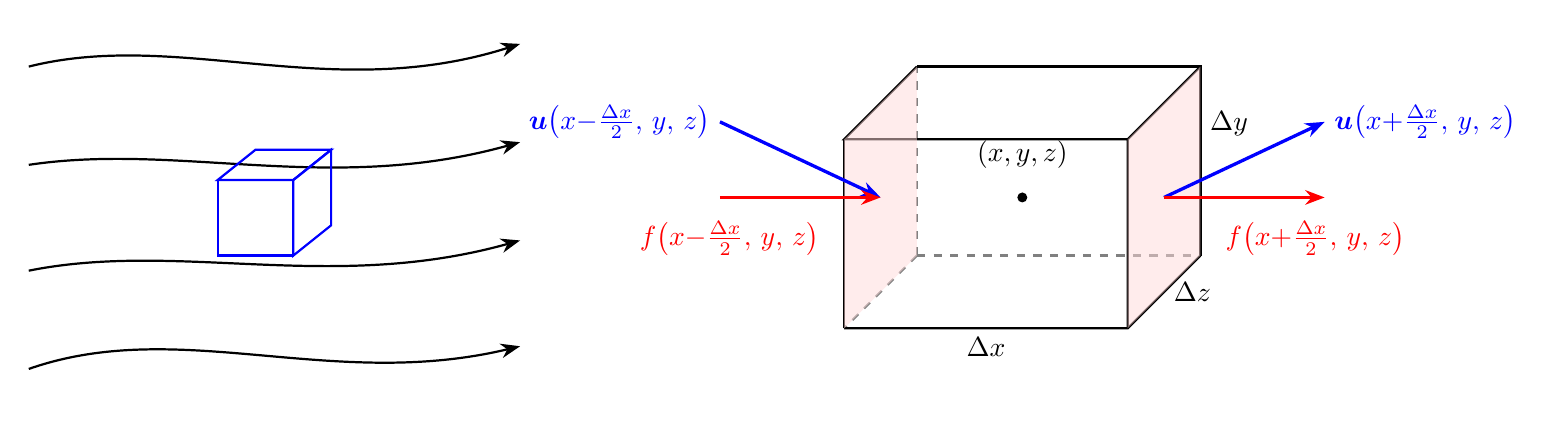
\begin{tikzpicture}[every node/.style={font=\normalsize}, scale=1.2]

  %% Left panel: flow with small box
  \begin{scope}[xshift=-7cm, scale=0.8]
    % Flow lines (curves with arrows)
    \draw[-{Stealth[length=7pt]}, thick]
      (-3,2.5) .. controls (-1,3.0) and (1,2.0) .. (3.5,2.8);
    \draw[-{Stealth[length=7pt]}, thick]
      (-3,1.2) .. controls (-1,1.5) and (1,0.8) .. (3.5,1.5);
    \draw[-{Stealth[length=7pt]}, thick]
      (-3,-0.2) .. controls (-1,0.2) and (1,-0.5) .. (3.5,0.2);
    \draw[-{Stealth[length=7pt]}, thick]
      (-3,-1.5) .. controls (-1,-0.8) and (1,-1.8) .. (3.5,-1.2);

    % Small 3D box (blue)
    \def\bx{-0.5} \def\by{0.0} % box center offset
    \def\bs{1.0} % box size
    % Front face
    \draw[thick, blue] (\bx,\by) -- +(\bs,0) -- +(\bs,\bs) -- +(0,\bs) -- cycle;
    % Top face
    \draw[thick, blue] (\bx,{\by+\bs}) -- +(\bs,0) -- +({\bs+0.5},0.4) -- +(0.5,0.4) -- cycle;
    % Right face
    \draw[thick, blue] ({\bx+\bs},\by) -- +(0.5,0.4) -- +(0.5,{\bs+0.4}) -- +(0,\bs) -- cycle;
  \end{scope}

  %% Right panel: detailed box with flux arrows
  % 3D box - back edges
  \draw[thick, dashed, gray] (0,0,0) -- (3,0,0);
  \draw[thick, dashed, gray] (0,0,0) -- (0,2,0);
  \draw[thick, dashed, gray] (0,0,0) -- (0,0,2);

  % 3D box - front edges
  \draw[thick] (3,0,0) -- (3,2,0) -- (0,2,0);
  \draw[thick] (3,0,0) -- (3,0,2) -- (0,0,2);
  \draw[thick] (0,2,0) -- (0,2,2) -- (3,2,2) -- (3,0,2);
  \draw[thick] (3,2,0) -- (3,2,2);
  \draw[thick] (0,0,2) -- (0,2,2);

  % Left face (semi-transparent)
  \fill[red!15, opacity=0.5] (0,0,0) -- (0,2,0) -- (0,2,2) -- (0,0,2) -- cycle;
  % Right face (semi-transparent)
  \fill[red!15, opacity=0.5] (3,0,0) -- (3,2,0) -- (3,2,2) -- (3,0,2) -- cycle;

  % Left side: u enters the box, endpoint at face center (0,1,1)
  \draw[-{Stealth[length=7pt]}, very thick, blue] (-1.7,1.8,1) -- (0,1,1);
  \node[blue, left] at (-1.7,1.8,1) {$\boldsymbol{u}\!\left(x{-}\frac{\Delta x}{2},\, y,\, z\right)$};
  % f component (red, horizontal/perpendicular to face, same x-length as blue)
  \draw[-{Stealth[length=7pt]}, very thick, red] (-1.7,1,1) -- (0,1,1);
  \node[red, below] at (-1.6,0.85,1) {$f\!\left(x{-}\frac{\Delta x}{2},\, y,\, z\right)$};

  % Right side: u exits the box, startpoint at face center (3,1,1)
  \draw[-{Stealth[length=7pt]}, very thick, blue] (3,1,1) -- (4.7,1.8,1);
  \node[blue, right] at (4.7,1.8,1) {$\boldsymbol{u}\!\left(x{+}\frac{\Delta x}{2},\, y,\, z\right)$};
  % f component (red, horizontal/perpendicular to face, same x-length as blue)
  \draw[-{Stealth[length=7pt]}, very thick, red] (3,1,1) -- (4.7,1,1);
  \node[red, below] at (4.6,0.85,1) {$f\!\left(x{+}\frac{\Delta x}{2},\, y,\, z\right)$};

  % Labels
  \node[below] at (1.5,0,2) {$\Delta x$};
  \node[right] at (3,0,1) {$\Delta z$};
  \node[right] at (3,1.4,0) {$\Delta y$};

  % Center point
  \fill (1.5,1,1) circle (1.5pt);
  \node[above] at (1.5,1.2,1) {$(x,y,z)$};
\end{tikzpicture}
\end{document}
